\section{Exploration numérique}
Cette partie regroupe les réponses aux questions 1 à 7 de l'énoncé, réalisées à l'aide du programme \texttt{Markov Graph Analyzer} développé en C \parencite{markovGraphAnalyzer2025}.

\subsection{Approche de calcul}
\begin{itemize}[label=\textbullet]
  \item Charger la matrice de transition \texttt{input\_data/matrix.txt} et vérifier que chaque ligne somme à 1.
  \item Implémenter la propagation \(\Pi^{(n)} = \Pi^{(0)} P^{n}\) et tracer \(n \mapsto \Pi^{(n)}\) pour repérer les convergences/oscillations.
  \item Conserver les scripts et commandes utilisés (à déposer en annexe ou référencés depuis un dépôt).
\end{itemize}

\subsection{Scénarios et résultats attendus}
Pour chaque configuration initiale ci-dessous, documenter : (i) les vecteurs \(\Pi^{(n)}\) pour \(n=1,2,10,50\), (ii) les graphes de convergence, (iii) l'existence et la valeur éventuelle de la distribution limite.

\subsubsection{Question 1 — départ en état 2}
Le système part de l’état \(2\) (\(\Pi^{(0)} = e_2\)). Les calculs numériques ont été effectués avec le programme \texttt{./markov-graph-analyzer ---in data/from\_moodle/matrix.txt ---eps 0.01 ---dist-start 2 ---dist-steps 50}, basé sur la fonction \texttt{dist\_power}\textsuperscript{\ref{lst:dist_power}}.
Les distributions non nulles restent confinées dans la classe finale \(C_2=\{5,12,21,25,2\}\); toutes les autres composantes restent nulles (chaîne réductible, classe fermée car pas de successeurs).

\begin{figure}[H]
  \centering
  \includegraphics[width=0.7\textwidth]{hasse_q1.png}
  \caption{Diagramme de Hasse des classes communicantes (export du programme).}
  \label{fig:q1_hasse}
\end{figure}

\paragraph{(a) Distributions demandées.} Pour \(n=1,2,10,50\), seules les cinq composantes de \(C_2\) sont non nulles (la somme vaut 1 à chaque étape). On obtient le tableau (valeurs non nulles uniquement) :

\begin{table}[H]
  \centering
  \begin{tabular}{@{}lccccc@{}}
    \toprule
    \(n\) & \(\Pi^{(n)}(2)\) & \(\Pi^{(n)}(5)\) & \(\Pi^{(n)}(12)\) & \(\Pi^{(n)}(21)\) & \(\Pi^{(n)}(25)\) \\
    \midrule
    1  & 0.30   & 0.20   & 0.40   & 0.00   & 0.10   \\
    2  & 0.23   & 0.22   & 0.28   & 0.17   & 0.10   \\
    10 & 0.2397 & 0.1953 & 0.2338 & 0.1796 & 0.1516 \\
    50 & 0.2397 & 0.1953 & 0.2338 & 0.1796 & 0.1516 \\
    \bottomrule
  \end{tabular}
  \caption{Distributions \(\Pi^{(n)}\) (départ en \(e_2\)), données issues de \texttt{data/q1/n\{1,2,10,50\}\_out.txt}.}
  \label{tab:q1_distributions}
\end{table}

\paragraph{(b) Graphe \(n \mapsto \Pi_A(n)\).} La figure~\ref{fig:q1_pi} trace les cinq composantes non nulles pour \(n \in \{1,2,10,50\}\) (les autres restent à 0), avec un axe des abscisses en échelle logarithmique (base 10) pour mettre en évidence les premiers pas et les itérations lointaines.
On observe un lissage rapide vers la stationnaire autour de \(n\approx 10\).

\begin{figure}[H]
  \centering
  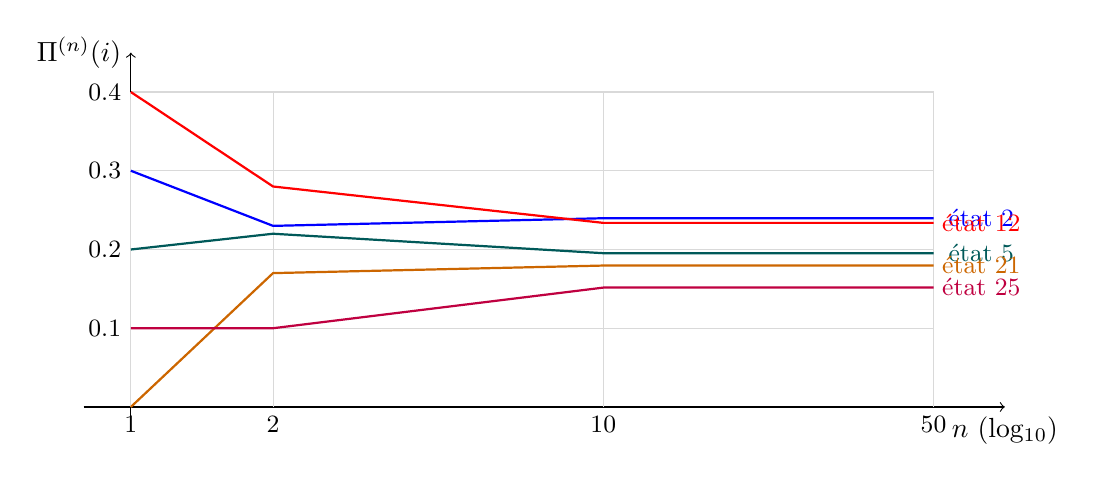
\begin{tikzpicture}[xscale=6,yscale=10]
    % Axes
    \draw[->] (-0.1,0) -- (1.85,0) node[below] {$n$ (log\textsubscript{10})};
    \draw[->] (0,-0.02) -- (0,0.45) node[left] {$\Pi^{(n)}(i)$};
    % Grille et repères (log10)
    \foreach \x/\lbl in {0/{\small 1},0.3010/{\small 2},1/{\small 10},1.6990/{\small 50}}{
      \draw[gray!30] (\x,0) -- (\x,0.4);
      \node[below] at (\x,0) {\lbl};
    }
    \foreach \y in {0.1,0.2,0.3,0.4}{\draw[gray!30] (0,\y) -- (1.7,\y); \node[left] at (0,\y) {\small \y};}
    % Etat 2
    \draw[blue,thick] plot coordinates {(0,0.3) (0.3010,0.23) (1,0.2397) (1.6990,0.2397)};
    \node[blue] at (1.8,0.24) {\small état 2};
    % Etat 12
    \draw[red,thick] plot coordinates {(0,0.4) (0.3010,0.28) (1,0.2338) (1.6990,0.2338)};
    \node[red] at (1.8,0.234) {\small état 12};
    % Etat 5
    \draw[teal!70!black,thick] plot coordinates {(0,0.2) (0.3010,0.22) (1,0.1953) (1.6990,0.1953)};
    \node[teal!70!black] at (1.8,0.196) {\small état 5};
    % Etat 21
    \draw[orange!80!black,thick] plot coordinates {(0,0.0) (0.3010,0.17) (1,0.1796) (1.6990,0.1796)};
    \node[orange!80!black] at (1.8,0.18) {\small état 21};
    % Etat 25
    \draw[purple,thick] plot coordinates {(0,0.1) (0.3010,0.1) (1,0.1516) (1.6990,0.1516)};
    \node[purple] at (1.8,0.152) {\small état 25};
  \end{tikzpicture}
  \caption{Évolution des composantes non nulles \(\Pi^{(n)}(i)\) (départ en \(e_2\)).}
  \label{fig:q1_pi}
\end{figure}

\paragraph{(c) Existence et valeur de la distribution limite.}
\begin{itemize}[label=\textbullet]
  \item \(C_2\) est fermée : aucune probabilité ne s’échappe vers les autres classes, donc toute la masse reste dans \(\{5,12,21,25,2\}\).
  \item Les états de \(C_2\) communiquent et l’on peut y revenir après plusieurs pas sans être bloqué dans un cycle rigide ; en répétant les pas, la masse s’y « mélange ».
  \item Ce mélange se stabilise numériquement vers un seul profil : partir de l’état 2 (ou de n’importe quel état de \(C_2\)) conduit au même vecteur limite.
\end{itemize}
Les valeurs limites sont obtenues numériquement par la fonction \texttt{stationary\_distribution}\textsuperscript{\ref{lst:stationary}} du programme \texttt{./markov-graph-analyzer}, appliquée à la sous-matrice de la classe persistante.
Sur les 27 états, la limite vaut
\[
  \Pi^{(\infty)}(5)=0{,}1944,\quad
  \Pi^{(\infty)}(12)=0{,}2332,\quad
  \Pi^{(\infty)}(21)=0{,}1806,\quad
  \Pi^{(\infty)}(25)=0{,}1520,\quad
  \Pi^{(\infty)}(2)=0{,}2398,
\]
et est nulle ailleurs. Les valeurs observées à \(n=10\) et \(n=50\) coïncident avec cette limite à \(10^{-4}\) près.

\subsubsection{Question 2 — répartition uniforme sur 2, 5, 12, 21, 25}
\placeholder{Analyser la convergence avec les poids initiaux égaux.}

\subsubsection{Question 3 — répartition aléatoire sur 2, 5, 12, 21, 25}
\placeholder{Étudier la sensibilité de la distribution limite aux paramètres \(a,b,c,d,e\).}

\subsubsection{Question 4 — états 8, 9, 16}
\placeholder{Comparer départ en 8 vs. mélange uniforme vs. mélange aléatoire.}

\subsubsection{Question 5 — états 10, 14, 19, 22, 24}
\placeholder{Identifier les comportements limites selon les trois répartitions demandées.}

\subsubsection{Question 6 — états 6, 17, 20}
\placeholder{Documenter les trajectoires de \(\Pi^{(n)}\) et la présence/absence de limite.}

\subsubsection{Question 7 — états 3, 7, 23}
\placeholder{Même analyse : convergence éventuelle et dépendance à l'initialisation.}

\subsection{Visualisations suggérées}
\begin{itemize}[label=\textbullet]
  \item Graphes de barres superposées montrant \(\Pi^{(n)}\) pour quelques valeurs de \(n\).
  \item Courbes de \(\ell_1\)-distance entre \(\Pi^{(n)}\) et la distribution limite candidate.
  \item Schémas de graphe (TikZ) pour les sous-chaînes explorées, si pertinents.
\end{itemize}
